\documentclass[../../../topic_machine-learning]{subfiles}

\begin{document}

\sectionline
\section{勾配降下法}

逐次的にパラメータを更新していくアプローチの中で、\keyword{勾配}の情報を使ってパラメータを逐次的に更新する方法を\keywordJE{勾配降下法}{GE: gradient descent}という。

\subsection{勾配と関数の値}

目的関数$L(\vb*{\theta})$の、$\vb*{\theta}$に関する勾配
\begin{equation*}
  \nabla L(\vb*{\theta}) = \frac{\partial L}{\partial \vb*{\theta}} = \left( \frac{\partial L}{\partial \theta_1}, \ldots, \frac{\partial L}{\partial \theta_n} \right)
\end{equation*}
は、$\vb*{\theta}$を変化させたときに関数の値が最も急激に増加する方向を表している。

そして、その逆$-\nabla L(\vb*{\theta})$が、関数の値を最も急激に下げる方向を表している。

\begin{supplnote}
  勾配がなぜ関数の値を最も急激に増加させる方向を表すのかは、拙著「\webbookA」で解説している。
\end{supplnote}

\subsection{勾配降下法のアルゴリズム}

勾配降下法では、現在のパラメータに関する勾配$\vb*{v} = \nabla L$を計算し、その逆方向にパラメータを更新する。
\begin{equation*}
  \vb*{\theta}' = \vb*{\theta} - \eta \vb*{v} \quad (\eta > 0)
\end{equation*}

ここで、$\eta$は\keyword{学習率}と呼ばれるハイパーパラメータであり、更新の大きさを微調整するために用いる。

\br

そして、更新後のパラメータ$\vb*{\theta}'$を新たなパラメータとして、再び勾配を計算し、同様に更新を繰り返していく。
あらかじめ決めた回数に達するまで、もしくは、目的関数の改善幅が閾値を下回るまで、更新を続ける。

\subsection{学習率と収束}

勾配は局所的な関数値の変化を表しており、遠くの地形の情報はわからない。

そのため、少しずつ山を下っていくのが勾配降下法の基本的な考え方である。

\br

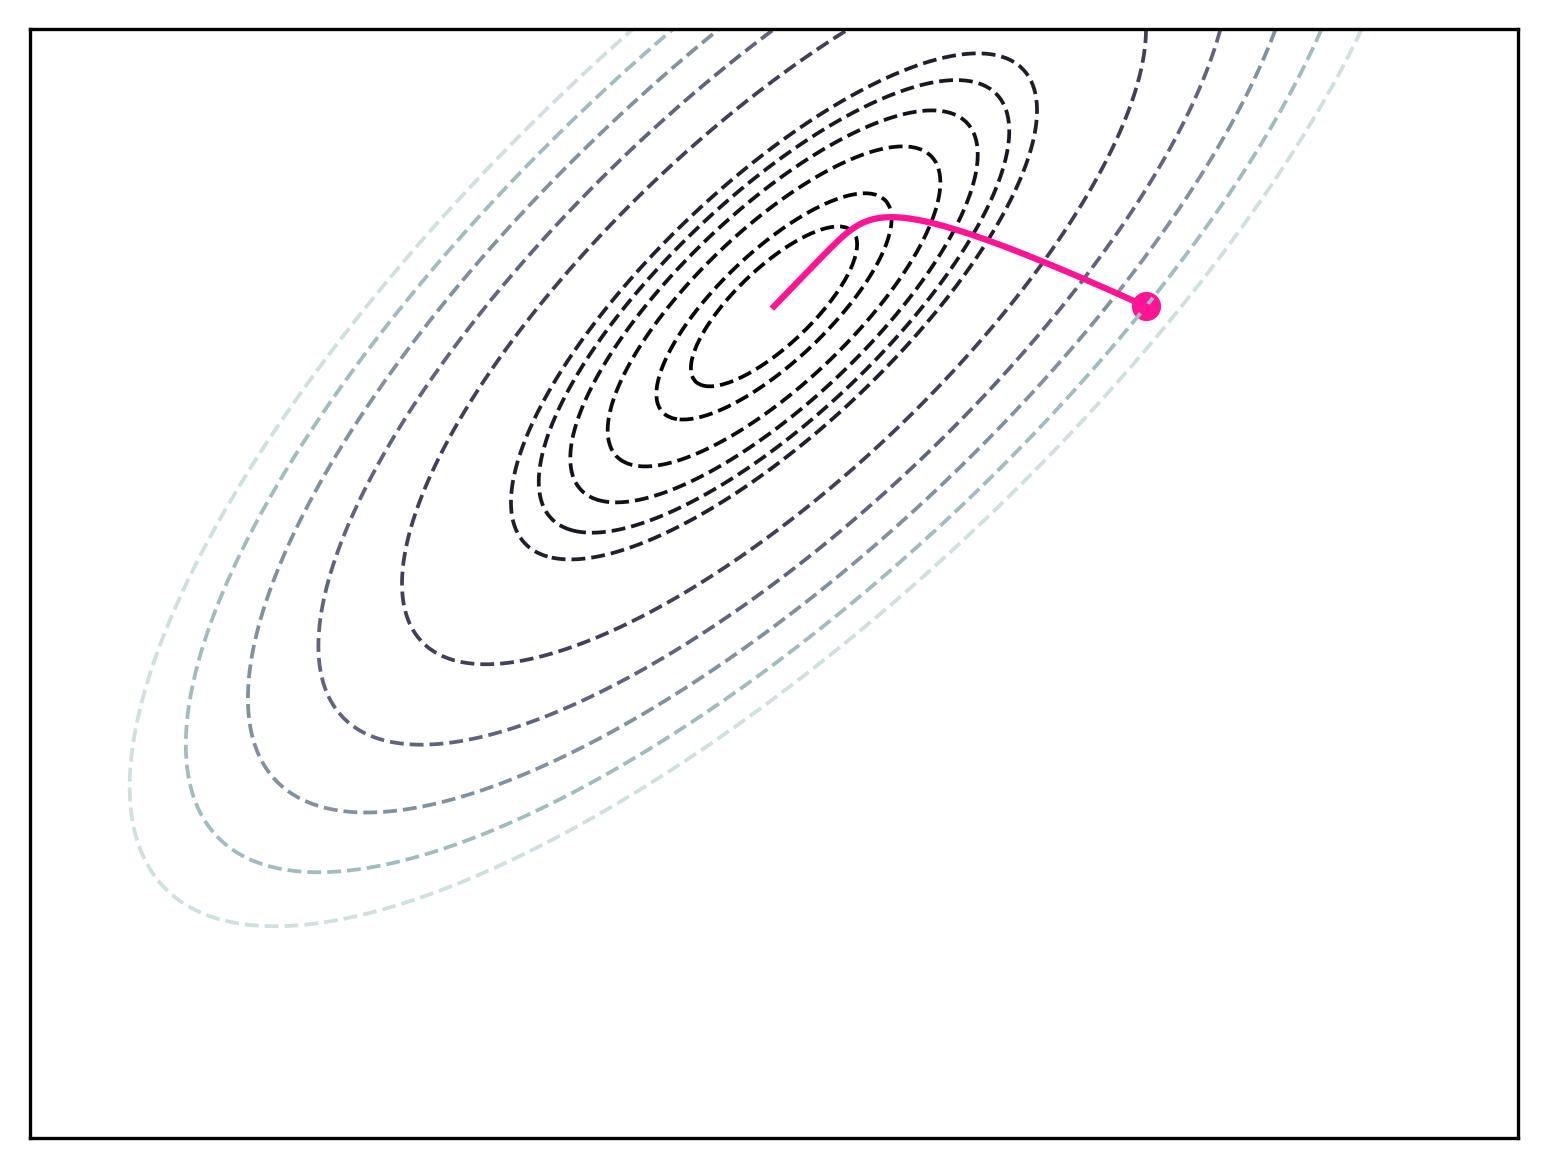
\includegraphics[width=0.75\linewidth]{./python/gradient-descent.png}

ここで、学習率$\eta$を大きくしすぎると、一気に谷を飛び越えてしまう。

この場合、無駄な移動が発生して収束に時間がかかったり、最適解にたどり着けなくなる(収束しない)可能性がある。

\br

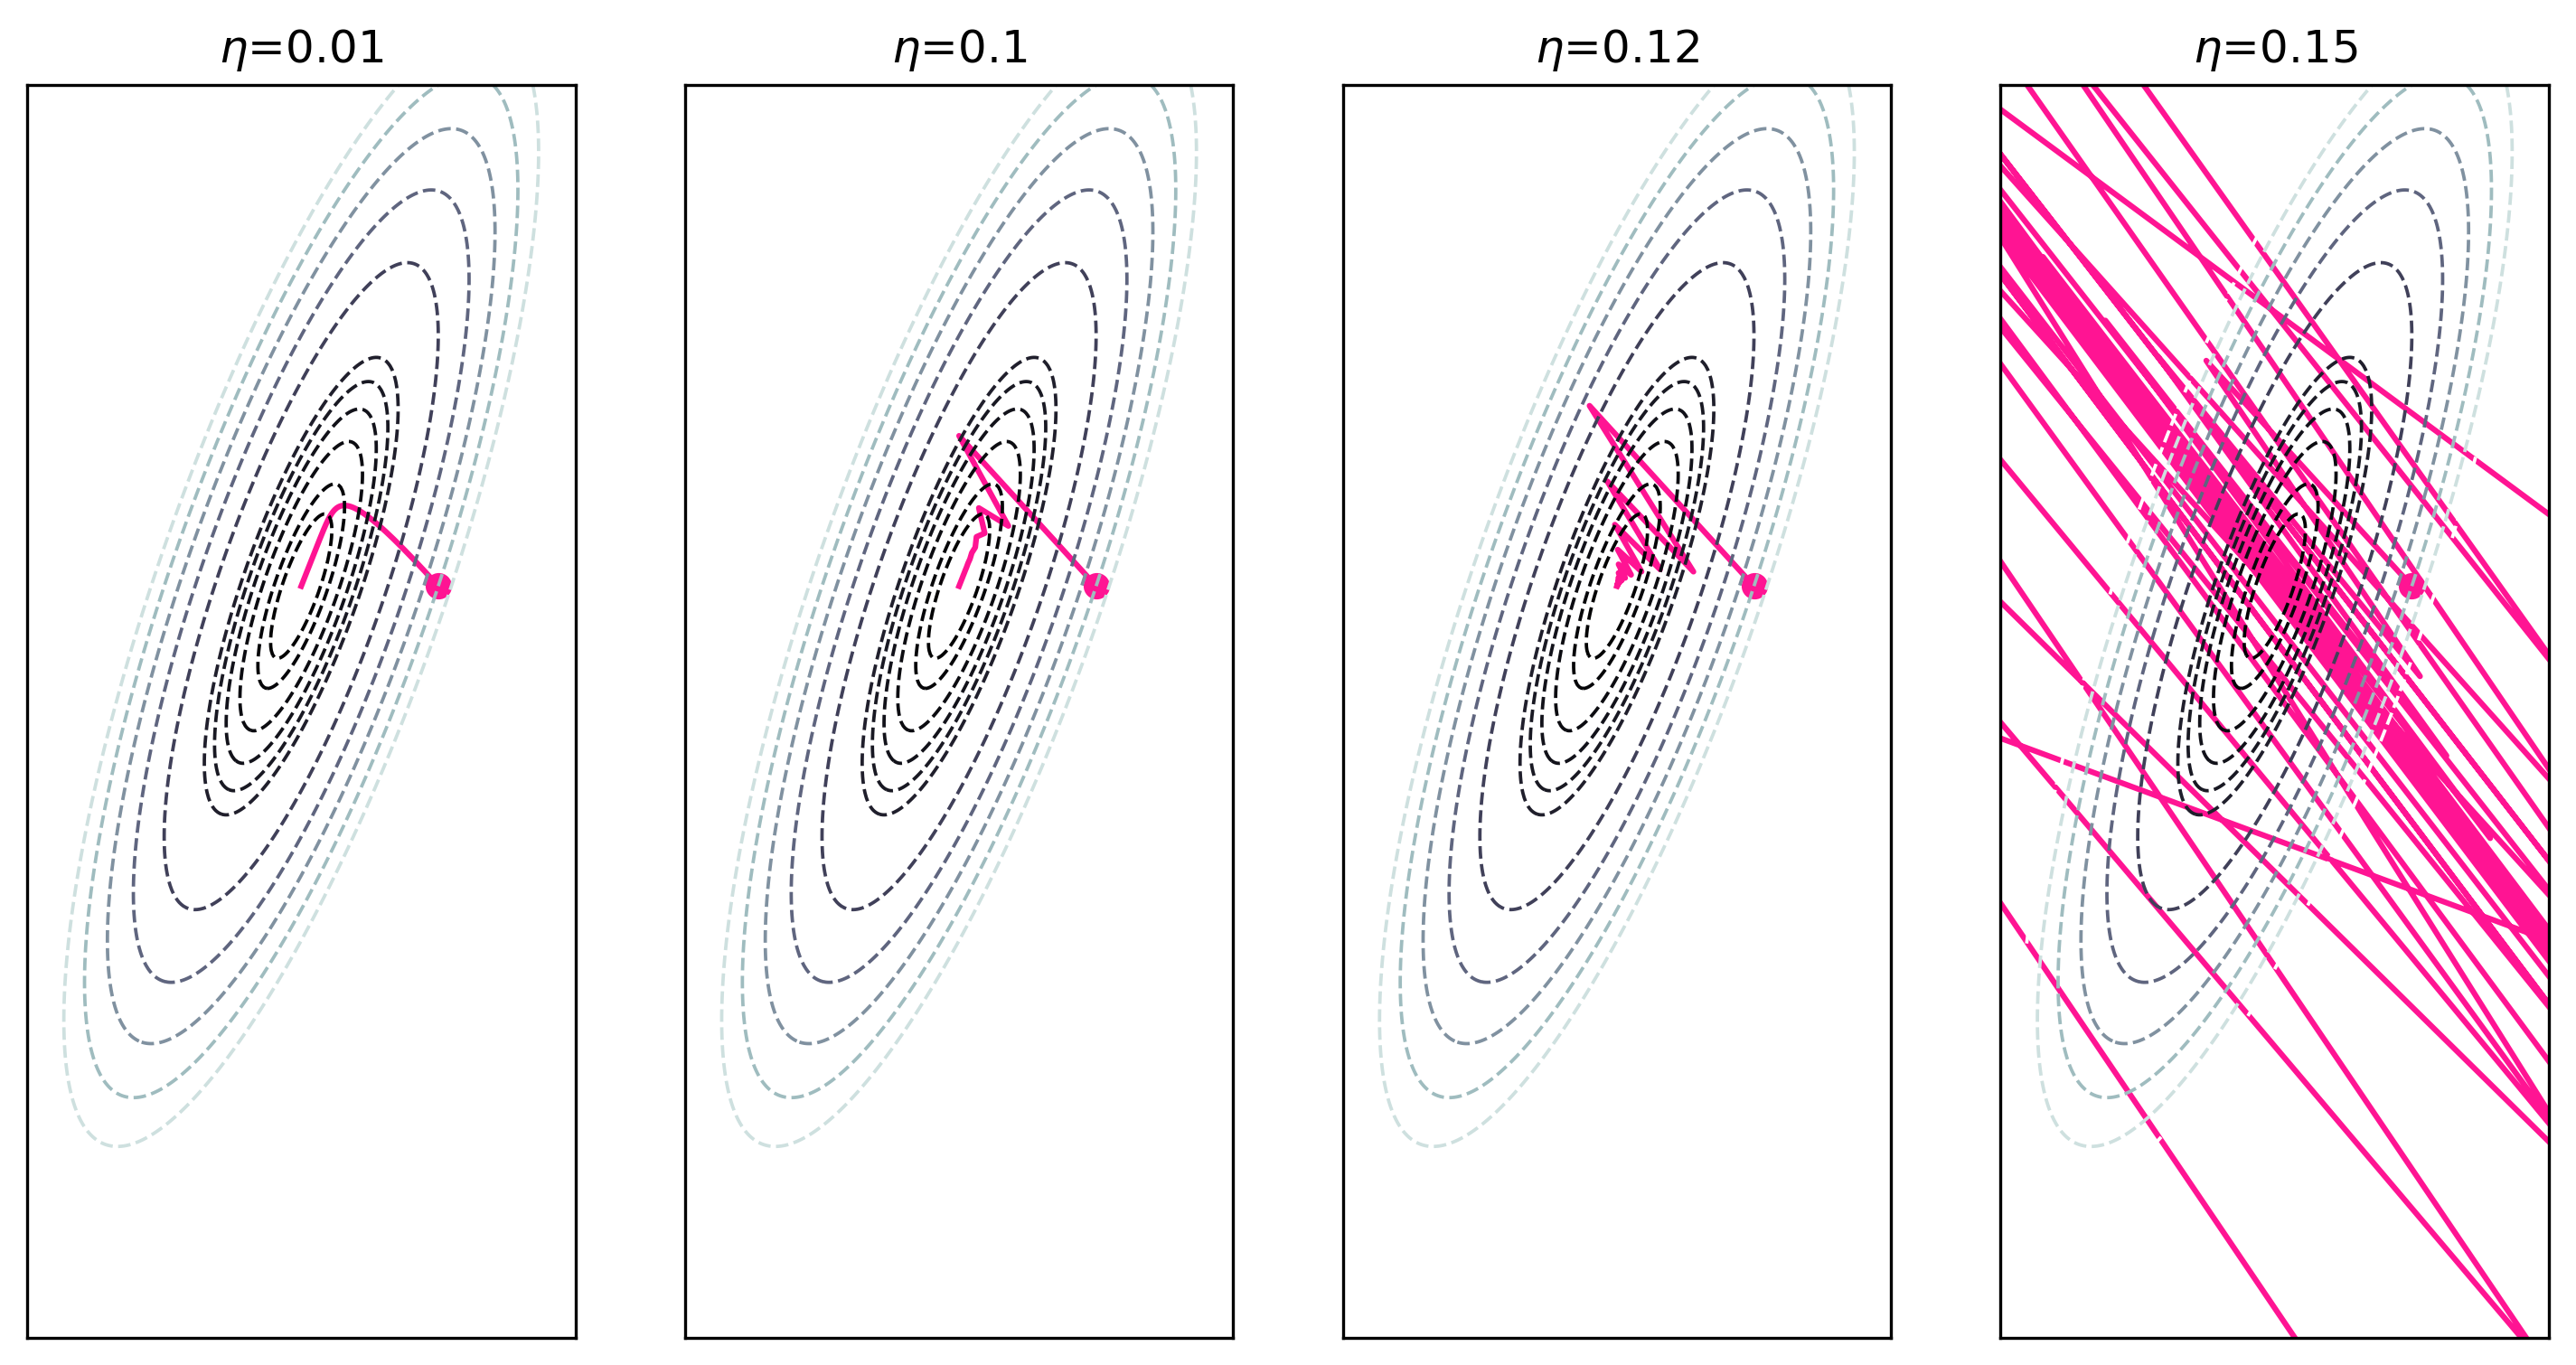
\includegraphics[width=0.95\linewidth]{./python/gradient-descent_compare-alpha.png}

一方で、学習率$\eta$が小さければ小さいほど、狭い歩幅で山を下っていくようなもので、その分収束に時間がかかってしまう。

\subsection{勾配降下法の計算コスト}

勾配降下法は、すべてのパラメータ$\theta_1, \ldots, \theta_n$をまとめて更新できるため、効率が良い。

\br

しかし、勾配を計算するためには、毎回訓練データ全体を走査する必要がある。

なぜなら、次のように、現在のパラメータについての勾配は、各訓練データについての勾配の和であるからだ。
\begin{equation*}
  \nabla L(\vb*{\theta}) = \frac{\partial L}{\partial \vb*{\theta}} = \frac{\partial}{\partial \vb*{\theta}} \left( \frac{1}{N} \sum_{i=1}^{N} l(\vb*{x}_i, y_i; \vb*{\theta}) \right) = \frac{1}{N} \sum_{i=1}^{N} \frac{\partial l(\vb*{x}_i, y_i; \vb*{\theta})}{\partial \vb*{\theta}}
\end{equation*}

\br

そのため、訓練事例数が大きい場合、勾配降下法の計算コストは非常に大きくなってしまう。

\end{document}
